\documentclass[12pt,a4paper,twoside, inzynierska]{pwr_wmat_praca_dyplomowa}
% Ustawienia języka
\usepackage[utf8]{inputenc}

% Ustawienia odnośników i grafik
\usepackage{hyperref}
\usepackage{graphicx}
\graphicspath{ {./images/} }
\usepackage{booktabs} % dla ładniejszych linii w tabeli
\usepackage[margin=1in]{geometry}
% Matematyka

\usepackage{amssymb}
\usepackage{amsthm}
% Wskaźniki kodu (jeśli będą potrzebne)
\usepackage{listings}
\usepackage{xcolor}
\usepackage{float}
\usepackage{caption}
\captionsetup[figure]{skip=2pt} % Zmniejsz odstęp do 2pt; dostosuj wartość według potrzeb
\lstset{
	backgroundcolor=\color{white},
	basicstyle=\footnotesize\ttfamily,
	breaklines=true,
	frame=single
}

% Numeracja dwustopniowa dla tabel i rysunków
\usepackage{chngcntr}
\counterwithin{figure}{chapter}
\counterwithin{table}{chapter}
\usepackage{indentfirst} % Jeśli chcesz wcięcia również w pierwszym akapicie rozdziału
\setlength{\parindent}{17pt} % Ustawienie wcięcia na 0
\setlength{\parskip}{0em}
\autor{Jacek Hejke}

\tytul{Prognozowanie kursów kryptowalut z wykorzystaniem analizy technicznej i uczenia maszynowego} 
\tytulang{Forecasting cryptocurrency prices using technical analysis and machine learning}

\opiekun{Dr. inż Joanna Janczura}
\kierunekstudiow{Matematyka stosowana}
\kierunekstudiowang{Applied Mathematics}
\specjalnoscang{Theoretical Mathematics} 
\streszczenie{Niniejsza praca inżynierska koncentruje się na prognozowaniu cen kryptowalut przy użyciu analizy technicznej oraz metod uczenia maszynowego. Zastosowano różnorodne techniki, w tym sieci neuronowe, w celu efektywnego przewidywania cen.Wskaźniki techniczne zostały użyte jako dane wejsciowe do modelu uczenia maszynowego, by zwiększyć dokładność prognoz i maksymalizacji zysków. Wyniki eksperymentów na danych, takich jak serie cenowe Bitcoina, pokazują potencjał wykorzystania sztucznej inteligencji w dziedzinie prognozowania kryptowalut.}
\streszczenieang{This engineering thesis focuses on forecasting cryptocurrency prices using technical analysis and machine learning methods. Various techniques, including neural networks, have been applied to effectively predict prices. Technical indicators were used as input data for the machine learning model to enhance forecast accuracy and maximize profits. Experimental results on data such as Bitcoin price series demonstrate the potential of using artificial intelligence in the field of cryptocurrency forecasting.}

\slowakluczowe{kryptowaluty, analiza techniczna, Bitcoin, sieci neuronowe, prognoza ceny}  
\slowakluczoweang{Cryptocurrencies, technical analysis, Bitcoin, neural networks, price forecasting}
\theoremstyle{plain}
\newtheorem{theorem}{Twierdzenie}
\numberwithin{theorem}{chapter}
\newtheorem{lemma}[theorem]{Lemat} 
\newtheorem{corollary}[theorem]{Wniosek}
\newtheorem{fact}[theorem]{Fakt}
\theoremstyle{definition}
\numberwithin{theorem}{chapter}
\newtheorem{definition}[theorem]{Definicja} 
\newtheorem{example}[theorem]{Przykład}
\newtheorem{note}[theorem]{Uwaga}
\begin{document}
	\frontmatter
	\maketitle
	\mainmatter
\tableofcontents	
	
	% Wstęp
	\chapter{Wstęp}
	\section{Wprowadzenie do problematyki}
	
	Niniejsza praca inżynierska koncentruje się na prognozowaniu kursów kryptowalut, wykorzystując metodologie analizy technicznej oraz nowoczesne techniki uczenia maszynowego. Kryptowaluty, będące dynamicznie rozwijającym się rynkiem finansowym, wyróżniają się specyficznymi cechami, które odróżniają je od tradycyjnych aktywów, takich jak akcje, obligacje czy surowce.
	
	Kryptowaluty, charakteryzujące się dużą zmiennością i trudną przewidywalnością, stanowią wymagające, ale i obiecujące pole badawcze. Nieumiejętne inwestowanie na giełdzie kryptowalut może spowodować duże straty finansowe, ale z odpowiednią wiedzą może przynieść wysokie zyski. Książka pt.\emph{"Giełda podstawy inwestowania"} Adama Zaremby \hyperref[info2]{[2]}, gdzie omawiane są podstawy i strategie inwestowania na rynku akcji, wiedza o kryptowalutach i ich zmienności jest kluczowa dla osiągnięcia sukcesu na dynamicznie zmieniającym się rynku cyfrowych walut. Zmienność ta jest zarówno wyzwaniem, jak i szansą dla inwestorów oraz analityków, a także dla naukowców poszukujących skutecznych narzędzi do przewidywania przyszłych ruchów cen.
	
	Główne kryptowaluty, takie jak Bitcoin czy Ethereum, stanowią przedmiot zainteresowania nie tylko inwestorów indywidualnych, ale również instytucji finansowych, które dostrzegają w nich potencjalne źródło zysków. Jednak ich ogromna dynamika oraz wpływ licznych czynników zewnętrznych, takich jak polityka regulacyjna, rozwój technologii blockchain, czy zmieniające się preferencje użytkowników, powodują, że prognozowanie ich kursów jest szczególnie trudnym zadaniem.
	
	Klasyczne metody analizy finansowej, choć stosowane z powodzeniem w przypadku bardziej stabilnych aktywów, mogą okazać się niewystarczające w kontekście kryptowalut. Z pomocą jednak przychodzą nam dwie główne metody analizy kursów. Jedną z nich jest analiza fundamentalna, która odpowiada na pytanie \emph{„dlaczego?”} \hyperref[info1]{[1]}. i skupia się na badaniu wewnętrznej wartości aktywa, odpowiadając na pytanie, dlaczego dany projekt może odnieść sukces lub ponieść porażkę. Obejmuje analizę takich czynników jak technologia stojąca za kryptowalutą, zespół deweloperów, zastosowanie praktyczne oraz plany rozwoju projektu. Dodatkowo na analizę fundamentalną kryptowalut duży wpływ mają także czynniki makroekonomiczne, takie jak globalna polityka monetarna, inflacja czy regulacje prawne, które mogą znacząco kształtować popyt i podaż na rynku aktywów cyfrowych.
	
	Drugą analizą metod jest analiza techniczna, która odpowiada na pytanie \emph{„kiedy?”}. W książce pt. \emph{"Analiza techniczna w praktyce"} Krzysztofa Kochana \hyperref[info3]{[3]} możemy poznać wiele technik umożliwiających nam odpowiedź na to pytanie. Pozwala ona na badanie wzorców cenowych i identyfikację trendów w oparciu o dane historyczne. Analiza techniczna opiera się na założeniu, że ceny rynkowe podążają za określonymi schematami, które można wykorzystać do przewidywania przyszłych ruchów.
	
	Swoją przygodę z kryptowalutami zacząłem w 2020 roku, podczas trwania COVID-19. Wprowadzenie obostrzeń dotyczących przemieszczania się zapoczątkowało moje zainteresowanie tym tematem.
	
	Celem naszej pracy jest analiza wybranych wskaźników analizy technicznej, takich jak np: ruchoma średnia, wykresy świecowe, zniesienia Fibonacciego, czy oscylator stochastyczny oraz ich zastosowanie do predykcji kursów kryptowalut. Wskaźniki te zostaną następnie wykorzystane jako zmienne wejściowe do wybranych prognostycznych modeli uczenia maszynowego, w szczególności opartych o sieci neuronowe. Wyniki otrzymanych prognoz zostaną porównane w oparciu o miary dokładności prognoz oraz wielkość zysku.
	
	W pracy, oprócz wstępu i zakończenia, zawarte zostały pięć rozdziałów. Pierwszy z nich zawiera podstawy teoretyczne następujących pojęć: kryptowaluta, analiza techniczna i uczenie maszynowe. Każde z nich zostało dogłębnie opisane, w celu poszerzenia wiedzy na temat pracy inżynierskiej. Następny rozdział opisuje wskaźniki techniczne, które zostały wykorzystane jako dane wejściowe do modelu predykcyjnego. W trzecim rozdziale opisano metodę wykorzystaną do prognozowania cen kryptowalut. W rozdziale z wynikami przedstawiono końcowy wynik i analizę wyników. Na koniec pracy napisano wnioski dotyczące modelu.
	% Podstawy teoretyczne
	\chapter{Podstawy teoretyczne}
	
	W niniejszym rozdziale zostaną omówione kluczowe pojęcia i teorie niezbędne do zrozumienia zagadnień poruszanych w pracy. Przyjrzymy się trzem głównym obszarom wiedzy: analizie technicznej, kryptowalutom oraz uczeniu maszynowemu. Każdy z tych obszarów stanowi fundament dla późniejszych badań nad prognozowaniem kursów kryptowalut, które łączą w sobie elementy z tych różnych dziedzin. W kolejnych sekcjach szczegółowo omówimy podstawy teoretyczne każdego z tych obszarów, co pozwoli na lepsze zrozumienie i zastosowanie metod w dalszej części pracy.

	\section{Wprowadzenie do analizy technicznej}
	Analiza techniczna jest jednym z najczęściej stosowanych narzędzi do przewidywania cen aktywów, takich jak papiery wartościowe, akcje, obligacje, surowce czy kryptowaluty. Jej celem jest pomoc inwestorowi w podejmowaniu decyzji o wejściu lub wyjściu z rynku w optymalnym momencie. Główne założenia tej metody opierają się na przekonaniu, że wszystkie istotne informacje o danym aktywie są już uwzględnione w jego cenie, a ruchy cenowe podążają za powtarzalnymi wzorcami, które można zidentyfikować i wykorzystać do prognozowania. W przeciwieństwie do analizy fundamentalnej, która skupia się na ocenie wartości wewnętrznej aktywa (na przykład na podstawie sytuacji makroekonomicznej), analiza techniczna opiera się wyłącznie na danych historycznych, takich jak cena, wolumen i zmienność rynkowa.

	Głównym założeniem analizy technicznej jest fakt, że cena porusza się według ustalonego trendu, który moża przewidzieć na podstawie przeszłych danych. Traderzy i inwestorzy posługują się róznymi narzędziami, takimi jak wskaźniki techniczne, formacje świecowe i linie trendu. Są to narzędzia pozwalające przewidzieć przyszły kurs kryptowaluty, a także czas w jakim to nastąpi. Kluczowymi narzędziami do analizy techniczej są: średnia ruchoma, formacje świecowe, zniesienie fibonacciego i oscylatory stochastyczne. 
	
	Podsumowując, analiza techniczna to potężne narzędzie do oceny prawdopodobieństwa przyszłych cen aktywów. Pozwala traderom i inwestorom ocenić sytuację panującą na rynku, aby ułatwić podejmowanie decyzji o optymalnym momencie wejścia i wyjścia z inwestycji.

	\section{Wprowadzenie do kryptowalut}
	 Słowo \emph{„Kryptowaluta”} jest znane przez większość ludzi, lecz bywa różnie interpretowane. Definicji jest wiele, według wikipedii jest to \emph{ "rozproszony system księgowy bazujący na kryptografii, przechowujący informację o stanie posiadania w umownych jednostkach."}\hyperref[info4]{[4]}, według Investopedia \emph{"Kryptowaluta to cyfrowa lub wirtualna waluta zabezpieczona kryptografią, co prawie uniemożliwia fałszowanie lub podwójne wydawanie."}\hyperref[info4]{[4]}. My skupimy się jednak na definicji ze strony Forbes: \emph{"Kryptowaluta to rodzaj aktywa cyfrowego, które inwestorzy mogą kupować, sprzedawać i przechowywać na giełdach kryptowalutowych."}\hyperref[info4]{[4]}. Pierwsza kryptowaluta jaka się pojawiła jest to \emph{Bitcoin}, który został stworzony w 2009 roku przez anonimową osobę lub grupę osób pod pseudonimem Satoshi Nakamoto. Bitcoin został pierwszą kryptowalutą stworzoną w technologi Blockchain, tzn zdecentralizowany i rozproszony rejestr danych. W praktyce oznacza to łańcuch bloków, z których każdy zawiera zapis transakcji. Na rysunku \ref{fig:blockchain} możemy zobaczyć krok po kroku jak działa blockchain.
	
	\vspace{12pt} % Odstęp 12 punktów przed tabelą
	\begin{figure}[ht!]
		\centering
		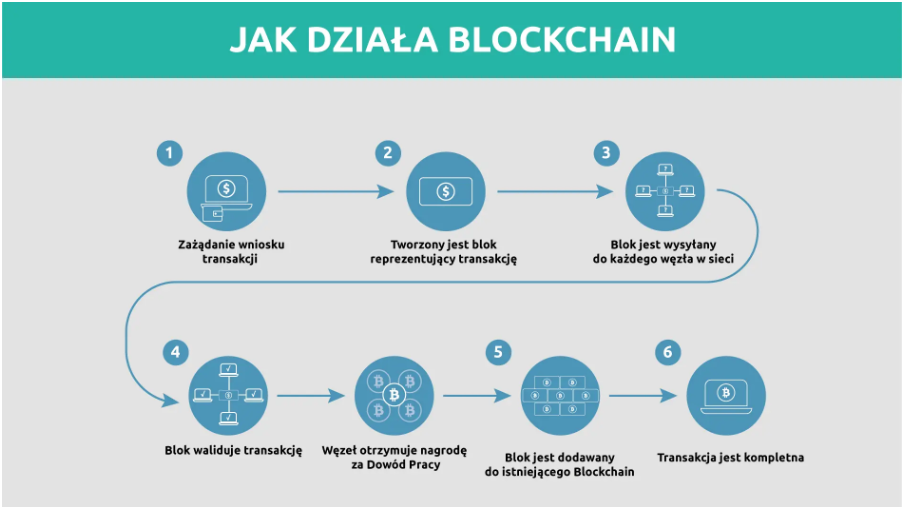
\includegraphics[width=\linewidth]{Jakdzialablockchain.png}
		\caption{Jak działa blockchain} % Tytuł centralnie nad tabelą
		\label{fig:blockchain}
		\textbf{Źródło:} \\
		\url{https://przemyslprzyszlosci.gov.pl/nawigator-technologiczny/blockchain/}
	\end{figure}
	\vspace{12pt} % Odstęp 12 punktów przed tabelą
	
	Każdy blok jest połączony z poprzednim w sposób kryptograficzny, tworząc łańcuch, którego nie da się w łatwy sposób zmodyfikować bez wpływu na całą strukturę \hyperref[info7]{[7]}. Dzięki tej technologii mamy zapewnione bezpieczeństwo i integralność danych, bez konieczności wykorzystywania centralnych instytucji, takich jak banki, do potwierdzenia transakcji.\newline
	Stworzenie Bitcoina spowodowało nowy początek w finansach, dla ludzi ceniących niezależność i wolność od wielkich instytucji finansowych, a także dało początek tworzeniu nowych kryptowalut. W kolejnych latach zostały stworzone nowe, tym razem już altcoiny, czyli alternatywne kryptowaluty do Bitcoina. Ethereum, jedna z najbardziej znanych i wpływowych altcoinów, została wprowadzona w 2015 roku przez Vitalika Buterina. Jego platforma umożliwia tworzenie zdecentralizowanych aplikacji (DApps) i inteligentnych kontraktów, co rozszerza możliwości technologii blockchain \hyperref[info9]{[9]}.\par
	Rozwój alternatywnych kryptowalut spowodował rozwój ekosystemu kryptowalut. Litecoin, na przykład, zaoferował szybsze czasy transakcji i inne algorytmy haszowania. Ripple (XRP) skupiło się na przyspieszeniu międzynarodowych płatności bankowych. Cardano stworzyło blockchain oparty na badaniach naukowych i recenzji naukowej (peer-review), co miało zapewnić jego większą skalowalność i bezpieczeństwo. Popularną monetą w darknecie stała się moneta Monero, gdyż jest skoncentrowana na prywatności. Umożliwia użytkownikom ukrycie informacji o transakcjach, co jest odpowiedzią na rosnące obawy dotyczące prywatności w cyfrowym świecie.\par
	Rosnącej popularności kryptowalut u ludzi nie mogły przeoczyć rządy i organy regulacyjne. Zaczęły się przyglądać nowym technologiom w tej dziedzinie, a co za tym idzie, wprowadzać regulacje i obostrzenia dotyczące kryptowalut. W niektórych krajach, takich jak Chiny, Algieria, Bangladesz czy Nepal, transakcje kryptowalutowe są nielegalne \hyperref[info8]{[8]}.\par
	W tamtym czasie popularne było kopanie kryptowalut \textit{(ang. mining)}, tzn. udostępnianie swojej mocy obliczeniowej z kart graficznych do weryfikacji i zatwierdzania transakcji w sieci blockchain oraz tworzenie nowych jednostek kryptowalut. W zamian otrzymywał nagrode w postaci krypto, którą kopał. Wielkość nagrody zależy od 2 czynników: hashrate i hashpower koparki. Niestety, w obliczu rosnącej popularności, trudność w wydobywaniu wzrosła, więc ludzie zaczeli łączyć się w pulach wydobywczych (mining pools). Dzięki zwiększonej wspólnej mocy obliczeniowej, zostaje zwiększona szansa na zdobycie większej nagrody.\hyperref[info10]{[10]}. Na obrazku (\ref{fig:kopaniekrypto}) jest przedstawiony w prosty sposób, jak to działa.\par
	Rozpowszechnienie kopania kryptowalut spowodowało znaczny wzrost cen kart graficznych na rynku. Ludzie masowo skupowali karty graficzne, aby zwiększyć zyski. Inwestycja była na tyle opłacalna, że koszty budowy zwracały się w pół roku. Dynamiczny rozwój górnictwa nie potrwał długo, ponieważ w 2022 roku Ethereum, czyli najbardziej dochodowa kryptowaluta do kopania, zmieniła swój algorytm z Proof of Work na Proof of Stake, co uniemożliwiło dalsze kopanie tej kryptowaluty. W rezultacie cena rynkowa kart GPU gwałtownie spadła. Część ludzi sprzedała koparki po kosztach, a część zaczęła kopać inne kryptowaluty działające na algorytmie Proof of Work.\par
	Podsumowując, kryptowaluty, jako zabezpieczone kryptografią cyfrowe środki wymiany, zrewolucjonizowały postrzeganie pieniądza i transakcji finansowych, wprowadzając nowe możliwości inwestycyjne i zapewniając większą prywatność. Od debiutu Bitcoina technologia blockchain poszerzyła swoje zastosowanie o inteligentne kontrakty i zdecentralizowane aplikacje, co stymulowało innowacje i tworzenie alternatywnych kryptowalut, takich jak Ethereum czy Monero. Regulacje i wyzwania technologiczne, w tym wpływ na środowisko związany z miningiem, stanowią kluczowe obszary zainteresowania regulatorów i twórców technologii. Mimo niepewności i zmienności, kryptowaluty nadal odgrywają istotną rolę w kształtowaniu przyszłości globalnych systemów finansowych i technologii.
	\vspace{12pt} % Odstęp 12 punktów przed tabelą
	\begin{figure}[H]
		\centering
		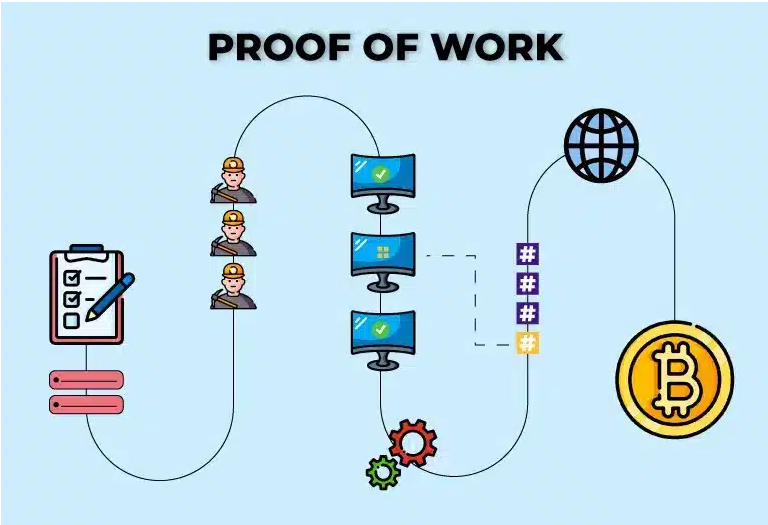
\includegraphics[width=0.8\linewidth]{kopaniekrypto.png}
		\caption{Schemat kopania kryptowalut} % Tytuł centralnie nad tabelą
		\label{fig:kopaniekrypto}
		\textbf{Źródło:} \\
		\url{https://businessinsider.com.pl/kryptowaluty/koparka-kryptowalut}
	\end{figure}
	\vspace{12pt} % Odstęp 12 punktów po tabeli
	
	\section{Wprowadzenie do uczenia maszynowego}
	W ostatnim czasie uczenie maszynowe stało się jednym z kluczowych obszarów w dziedzinie informatyki. Jego dynamiczny rozwój wpływa na wiele sektorów gospodarki, takich jak medycyna, przemysł, a także finanse, przynosząc innowacyjne rozwiązania i optymalizacje procesów. Uczenie maszynowe pozwala systemom komputerowym na samodzielne doskonalenie swoich działań poprzez analizę danych, bez potrzeby jednoznacznego programowania każdej czynności. \hyperref[info19]{[19]}
	
	Uczenie maszynowe to gałąź sztucznej inteligencji koncentrująca się na opracowywaniu algorytmów i modeli statystycznych, które umożliwiają komputerom uczenie się na podstawie danych. Zamiast polegać na sztywnych instrukcjach, systemy te identyfikują wzorce i zależności w zbiorach danych, co pozwala im na podejmowanie decyzji lub przewidywanie przyszłych zdarzeń. \hyperref[info19]{[19]}
	
	\subsection{Podstawowe pojęcia}
	
	Podstawowym celem uczenia maszynowego jest stworzenie modeli zdolnych do generalizacji, czyli poprawnego działania na nowych, nieznanych danych. Kluczowe pojęcia związane z tą dziedziną to:
	
	\begin{itemize} 
		\item \textbf{Model} — matematyczna reprezentacja procesu lub systemu, która jest trenowana na danych w celu wykonywania określonych zadań. 
		\item \textbf{Algorytm uczenia} — procedura, która dostosowuje parametry modelu na podstawie danych treningowych. 
		\item \textbf{Dane treningowe} — zestaw danych używany do nauki modelu, zawierający przykłady z odpowiednimi etykietami lub wynikami. 
		\item \textbf{Walidacja i testowanie} — procesy oceny wydajności modelu na danych niewidzianych podczas treningu. 
	\end{itemize}
	
	\subsection{Kluczowe rodzaje uczenia maszynowego \hyperref[info19]{[19]}} 
	\begin{itemize} 
		\item \textbf{Drzewa decyzyjne} — Struktury hierarchiczne, które reprezentują decyzje i ich możliwe konsekwencje.
		\item \textbf{Uczenie przez wzmacnianie} — Model (agent) uczy się optymalnej strategii działania poprzez interakcję ze środowiskiem i otrzymywanie nagród lub kar. Jest to podejście inspirowane psychologią behawioralną.
		\item \textbf{Uczenie nadzorowane} — W uczeniu nadzorowanym model jest trenowany na zbiorze danych wejściowych, którym przypisane są odpowiednie wyjścia (etykiety). Celem jest nauczenie modelu przewidywania poprawnych wyjść dla nowych danych.
		\item \textbf{Uczenie nienadzorowane} — Model otrzymuje jedynie dane wejściowe bez znanych etykiet. Celem jest odkrycie ukrytych struktur lub wzorców w danych. 
		\item \textbf{Sieci neuronowe} - Modele inspirowane biologicznymi sieciami neuronowymi, zdolne do modelowania złożonych nieliniowych zależności. Szczególną popularność zyskały \textbf{głębokie sieci neuronowe} w zastosowaniach takich jak rozpoznawanie obrazów czy przetwarzanie języka naturalnego.
	\end{itemize}

	\subsection{Zastosowania uczenia maszynowego w różnych dziedzinach \hyperref[info20]{[20]} } 
	Uczenie maszynowe ma szerokie zastosowanie w wielu sektorach. Przykładowe dziedziny to:
	\begin{itemize}
		\item  \textbf{Medycyna} — Diagnostyka wspomagana komputerowo, analiza obrazów medycznych, prognozowanie przebiegu chorób.
		\item  \textbf{Marketing} —  Personalizacja ofert, analiza zachowań klientów, segmentacja rynku.
		\item  \textbf{Transport} — Systemy autonomiczne, optymalizacja tras, zarządzanie flotą pojazdów.
		\item  \textbf{Energetyka} — Prognozowanie zużycia energii, zarządzanie sieciami energetycznymi, optymalizacja produkcji.
		\item  \textbf{Finanse} — Wykrywanie oszustw, analiza ryzyka, automatyzacja procesów kredytowych, predykcja wartości aktywów.
	\end{itemize}

	Uczenie maszynowe to dynamicznie rozwijająca się dziedzina, która znacząco wpływa na wiele aspektów naszego życia. Zrozumienie jej podstaw i wyzwań jest kluczowe dla skutecznego wykorzystania jej potencjału w przyszłości. 
	
	% Wybrane wskaźniki analizy technicznej
	\chapter{Wybrane wskaźniki analizy technicznej}
	W tym rozdziale skupimy się na wybranych wskaźnikach analizy technicznej, które są szeroko stosowane przez traderów na całym świecie. Przedstawimy zarówno teorie stojące za każdym z wskaźników, jak i praktyczne zastosowania, które pomagają w identyfikacji potencjalnych punktów wejścia i wyjścia z rynku.
	
	Rozpoczniemy od omówienia Średniej Ruchomej (\textit{Moving Average}), która pomaga wygładzić ceny aktywów, aby lepiej zrozumieć kierunki trendów. Następnie przejdziemy do Wzorów Świecowych (\textit{Candlestick Charts}), które dostarczają wglądu w emocje rynkowe i mogą sygnalizować nadchodzące zmiany w trendzie. Zniesienia Fibonacciego (Fibonacci Retracements) to kolejne narzędzie, które pozwala zidentyfikować potencjalne poziomy wsparcia i oporu na podstawie zasad matematycznych. Są to poziomy procentowe, które wskazują miejsca, gdzie cena może potencjalnie zatrzymać lub odwrócić swój poprzedni ruch. Typowo wykorzystywane procentowe poziomy zniesień to 23.6\%,\ 38.2\%,\ 50\%,\ 61.8\%,\ 78.6\%. Na koniec przyjrzymy się Oscylatorowi Stochastycznemu (Stochastic Oscillator), który jest używany do identyfikacji warunków nadkupienia i nadwyprzedaży, dając traderom wskazówki, kiedy rynek może być gotowy do odwrócenia trendu.
	
	Każdy z tych wskaźników przyczynia się do lepszego zrozumienia dynamiki rynku i pomaga w skuteczniejszym zarządzaniu portfelem inwestycyjnym. Dane, które są przetwarzane, dotyczą godzinowych cen Bitcoina na przestrzeni czterech lat, począwszy od początku 2020 roku do 14 października 2024 roku. Na rysunku \ref{eq:sma} przedstawiono przykładowe dane obejmujące następujące kolumny:
		\vspace{12pt} % Odstęp 12 punktów przed tabelą
	
	\begin{figure}[H]
		\centering
		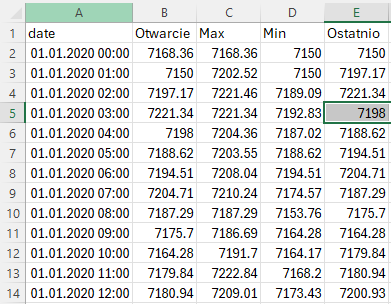
\includegraphics[width=0.7\textwidth]{excelkolumny.png}
		\caption{Przykładowe dane godzinowe dotyczące ceny Bitcoina}
		\label{fig:excelkolumny}
		\textbf{Źródło: Opracowanie własne}
	\end{figure}
	\vspace{12pt} % Odstęp 12 punktów po tabeli

	\begin{itemize}
		\item \textbf{data} -- Zawiera daty i godziny na które przypadały notowania.
		\item \textbf{Otwarcie} -- Cena "otwarcia" Bitcoina w danej godzinie.
		\item \textbf{Max} -- Najwyższa cena Bitcoina w ciągu godziny.
		\item \textbf{Min} -- Najniższa cena Bitcoin w ciągu godziny
		\item \textbf{Ostatnio} -- Cena "zamknięcia" Bitcoina w danej godzinie, która jest używana do obliczenia średniej ruchomej.
	\end{itemize}


	\section{Średnia ruchoma (\textit{ang. Moving Average})}

	\subsection{Opis wskaźnika}
	Średnia ruchoma to jeden z najpopularniejszych wskaźników używanych w analizie technicznej, stosowany do wygładzania krótkoterminowych fluktuacji cen i podkreślania długoterminowych trendów na rynku. Istnieją różne typy średnich ruchomych, z których najczęściej stosowane to średnia ruchoma prosta (\textit{ang. Simple Moving Average}, SMA), oraz średnia ruchoma wykładnicza (\textit{ang. Exponential Moving Average}, EMA). Każda z nich ma swoje specyficzne zastosowania. Przejdzmy teraz do szczegółowego opisania każdego z nich. \hyperref[info2]{[2]}
	
	\subsubsection{Średnia ruchoma prosta (\textit{ang. Simple Moving Average}) (SMA)}
	
	Średnia ruchoma prosta (SMA) jest obliczana jako średnia arytmetyczna cen zamknięcia instrumentu finansowego przez określony okres czasu. Jest to najprostsza forma średniej ruchomej, która nadaje każdej obserwacji równą wagę.  \hyperref[info2]{[2]}
	\begin{definition}  Średnia ruchoma prosta dana jest wzorem: \hyperref[info2]{[2]}
	\end{definition}
	\begin{equation} 
		\text{SMA}_{t} = \frac{\sum_{i=1}^{n} P_i}{n},
		\label{eq:sma} % Etykieta równania, dzięki której można się do niego odwołać
	\end{equation}
	gdzie \( P_i \) oznacza cenę zamknięcia w i-tym okresie, a \( n \) to liczba okresów.
	
	\subsubsection{Średnia ruchoma wykładnicza (\textit{ang. Exponential Moving Average}) (EMA)}
	
	Średnia ruchoma wykładnicza (EMA) kładzie większy nacisk na najnowsze dane, ale robi to w sposób wykładniczy. Jest ona bardziej skomplikowana w obliczeniu, ale reaguje szybciej na zmiany cen niż SMA.
	\hyperref[info2]{[2]}
	\begin{definition} 
	Wzór na średnią ruchomą wykładniczą można zapisać jako: \hyperref[info2]{[2]}
	\end{definition}
	\begin{equation}
		\text{EMA}_{t} = (P_i \times k) + (\text{EMA}_{t-1} \times (1 - k)),
		\label{eq:EMA}
	\end{equation}
	gdzie \( P_i \) to cena dzisiaj, a \( k \) to współczynnik wygładzania równy \( \frac{2}{n+1} \), przy czym \( n \) to liczba okresów. 
	\newline
	\subsection{Zastosowanie wskaźnika w analizie technicznej}
	
	
	\noindent \textbf{Identyfikacja trendu rynkowego}
	
	 Aby wyznaczyć trend rynkowy, potrzebujemy długoterminowej średniej kroczącej, tj. takiej, która jest mało wrażliwa na niewielkie zmiany ceny. Dobrym przykładem może być SMA 100-okresowa. Rysunek \ref{fig:SMA100} przedstawia przykładowy godzinowy wykres SMA100 dla danych BTC/USDT z przedziału czasowego od 17.08.2024 do 31.08.2024. Sygnał trendu wzrostowego możemy zauważyć, gdy cena przetnie wykres SMA100 od dołu. Może to być jednoznaczne z sygnałem kupna. Jeżeli cena przetnie wskaźnik od góry, mamy do czynienia z trendem spadkowym i sygnałem do sprzedaży aktywa. Dzięki zastosowaniu  średniej ruchomej, jesteśmy w stanie zidentyfikować trend rynkowy, a także generować sygnały kupna lub sprzedaży. \hyperref[info18]{[18]}
	
	\vspace{12pt}	
	\begin{figure}[H]
		\centering
		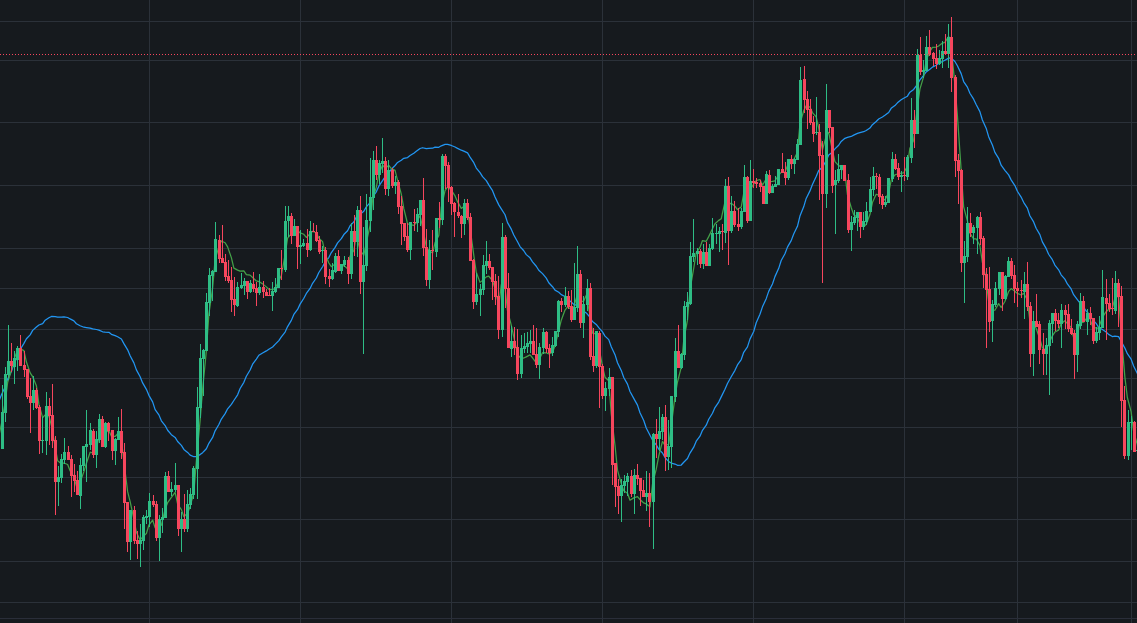
\includegraphics[width=1\textwidth]{SMA100.png}
		\caption{Przykład użycia SMA100 dla kryptowaluty BTC/USDT}
		\label{fig:SMA100}
		\textbf{Źródło: Opracowanie własne}
	\end{figure}
	\vspace{12pt}
	
	\noindent \textbf{Strategia:}
	
	 Najprostszym sygnałem do kupna/sprzedaży kryptowaluty jest przecięcie się krótkoterminowej SMA z długoterminową. Dzięki właściwościom krótkoterminowej SMA, jesteśmy w stanie lepiej podążać za ceną i szybciej reagować na zmiany ceny w porównaniu z długoterminową SMA, co nadaje się do prostej strategii. Przecięcie krótkoterminowej, np. SMA30, od dołu z długoterminową SMA100, generuje sygnał kupna. W przeciwnym wypadku, generuje sygnał sprzedaży. Na rysunku \ref{fig:SMA100i30} kolorem pomarańczowym narysowana jest SMA30, a niebieskim SMA100.	\hyperref[info18]{[18]} 
	
	\begin{figure}[H]
		\centering
		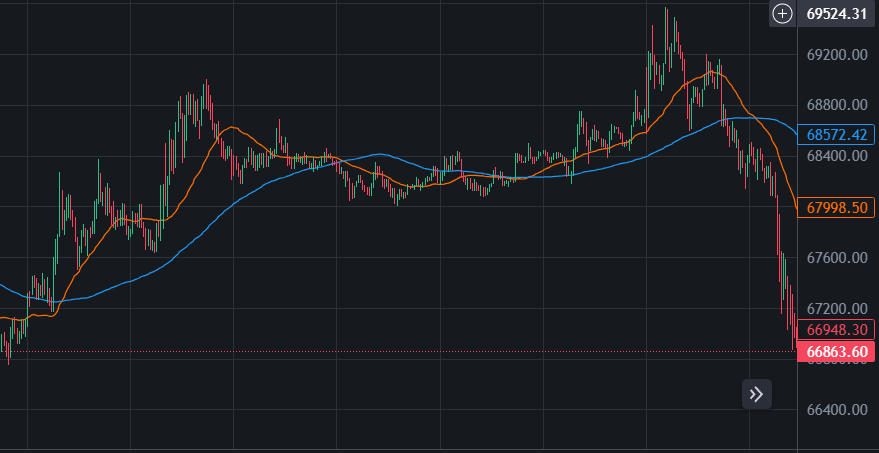
\includegraphics[width=1\textwidth]{SMA100i30.png}
		\caption{Przykład użycia SMA100 i SMA30 dla kryptowaluty BTC/USDT}
		\label{fig:SMA100i30}
		\textbf{Źródło: Opracowanie własne}
	\end{figure}
	\vspace{12pt}
		 
		
	\noindent \textbf{Średnia ruchoma wykładnicza}

	Drugą analizowaną średnią jest średnia ruchoma wykładnicza (EMA), która jest preferowana w strategiach wymagających szybkiego reagowania, jak day trading czy trading krótkoterminowy \hyperref[info3]{[3]}. EMA przypisuje większą wagę do najnowszych danych, co umożliwia jej szybkie dostosowanie się do zmian rynkowych. W przeciwieństwie do SMA, EMA lepiej radzi sobie z wygładzaniem wahania ceny, co czyni ją bardziej efektywną w przewidywaniu przyszłych ruchów cenowych \hyperref[info18]{[18]}. \newline

	\noindent \textbf{Strategia:}

	Sygnały kupna i sprzedaży można również generować przy pomocy przecięć dwóch średnich ruchomych wykładniczych. Przecięcie krótkoterminowej, np. EMA30, od dołu z długoterminową EMA100, generuje sygnał kupna. W przeciwnym wypadku, generuje sygnał sprzedaży. Rysunek \ref{fig:EMA30i100} przedstawia EMA30 kolorem pomarańczowym i EMA100 kolorem niebieskim.

	\begin{figure}[H]
		\centering
		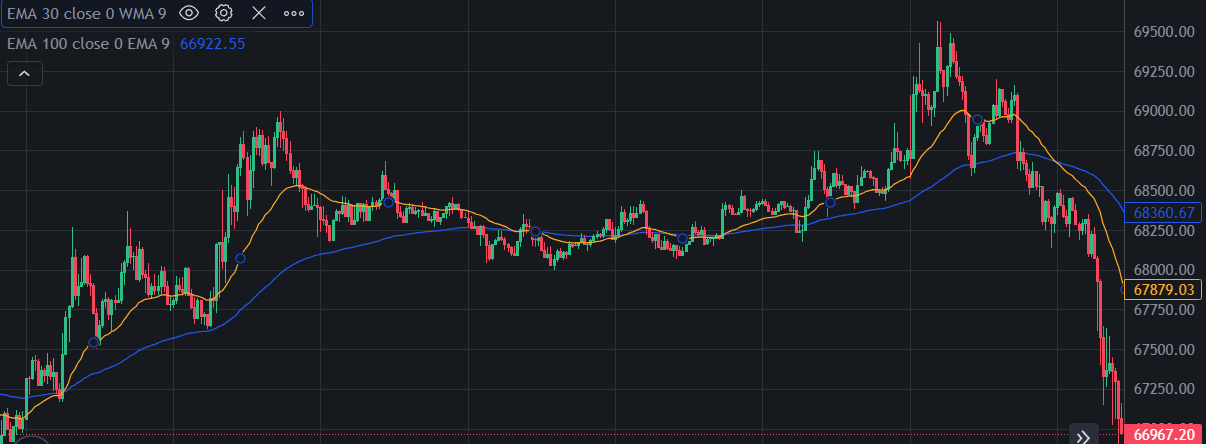
\includegraphics[width=1\textwidth]{EMA30i100.png}
		\caption{Przykład użycia EMA30 i EMA100 dla kryptowaluty BTC/USDT}
		\label{fig:EMA30i100}
		\textbf{Źródło: Opracowanie własne}
	\end{figure}
	\vspace{12pt}

		
	\noindent \textbf{Podsumowanie:}
	
	Porównując dwie średnie kroczące, nie jesteśmy w stanie stwierdzić, która jest lepsza. Wszystko zależy od przyjętej strategii inwestycyjnej. EMA jest lepiej dostosowana do krótkoterminowych transakcji, natomiast SMA do długoterminowych. Porównując obie średnie na jednym wykresie, możemy w prosty sposób zaobserwować ich zachowanie. Rysunek \ref{fig:EMAiSMA}  przedstawia zachowanie SMA15 i EMA15. Linią niebieską oznaczono SMA15, a linią białą – EMA15. Jak widzimy, EMA jest bardziej podatna na fluktuacje cen w porównaniu z SMA.
	\begin{figure}[H]
		\centering
		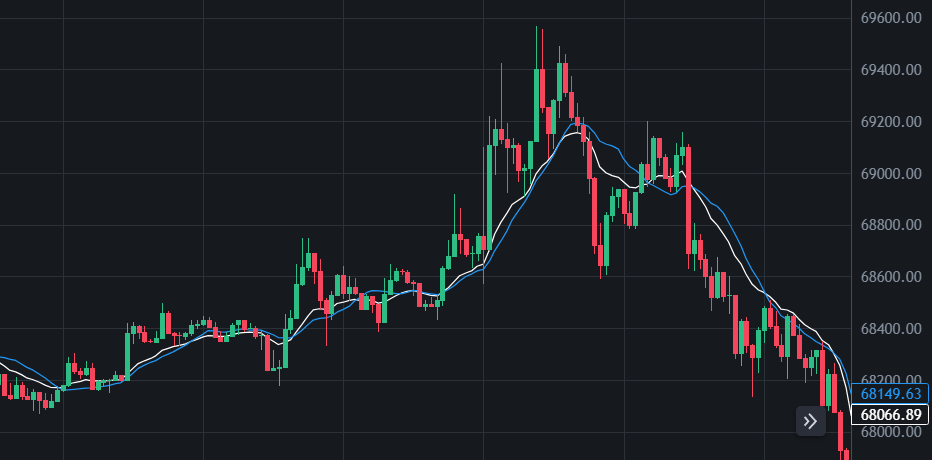
\includegraphics[width=1\textwidth]{EMAiSMA.png}
		\caption{Przykład użycia SMA15 i EMA15 dla kryptowaluty BTC/USDT}
		\label{fig:EMAiSMA}
		\textbf{Źródło: Opracowanie własne}
	\end{figure}
	\vspace{12pt}
	

	\section{Wykresy świecowe (\textit{ang. Candlestick Charts})}
	
	Wykres świecowy jest jedną z trzech metod, obok wykresu liniowego i słupkowego, służących do wizualizacji cen kryptowalut, ale także akcji, obligacji i innych aktywów \hyperref[info2]{[2]}. Przyjmuje się, że wynalazł go Munehisa Homma, japoński kupiec handlujący ryżem w XVIII wieku. Do Europy dotarła dość późno, dopiero pod koniec lat 90. XX wieku, i od tego czasu zyskała ogromną popularność. Większość analityków i profesjonalnych inwestorów opiera się na wykresie świecowym w celu identyfikacji trendów i przewidywania przyszłych ruchów cenowych \hyperref[info13]{[13]}.\newline
	
	\subsection{Charakterystyka wzorów świecowych}
	Wykresy świecowe są głównymi narzędziami do wizualizacji cen kryptowalut. W zależności od horyzontu czasowego pokazują nam za pomocą świecy, jak cena sie kształtowała. Głównymi horyzontami czasu jakie są używane to 15m, 1h, 4h, 1D. To oznacza, że jeżeli został wybrany horyzont czasowy 1h, to jedna świeca oznacza jedną godzinę \hyperref[info11]{[11]}. Główne parametry, jakie możemy odczytać ze świecy to (Rysunek \ref{fig:swieca}):
	\begin{itemize}
		\item \textbf{Upper Shadow (Górny knot)} -- Linia wychodząca z górnej części ciała świecy, reprezentuje maksymalną cenę (High) osiągniętą w danym okresie.
		\item \textbf{Real Body (Ciało)} -- Grubsza część świecy, która pokazuje różnicę pomiędzy ceną otwarcia (Open) a ceną zamknięcia (Close). Kolor ciała świecy wskazuje na kierunek ruchu cen: czerwony dla spadku, zielony dla wzrostu.
		\item \textbf{Lower Shadow (Dolny knot)} -- Linia wychodząca z dolnej części ciała świecy, reprezentuje minimalną cenę (Low) osiągniętą w danym okresie.
	\end{itemize}
	\vspace{12pt}
	\begin{figure}[H]
		\centering
		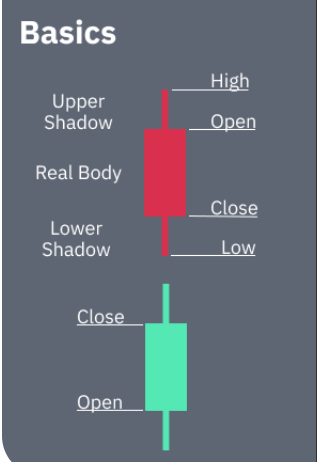
\includegraphics[width=0.5 \textwidth]{swieca.png}
		\caption{Budowa świecy}
		\label{fig:swieca}
		\textbf{Źródło:} \\
		\url{https://academy.binance.com/pl/articles/how-to-read-the-most-popular-crypto-candlestick-patterns}
	\end{figure}
	\vspace{12pt}
	\subsection{Przykładowe formacje i ich interpretacje}
	Analizując poszczególne wzorce świecowe, jesteśmy w stanie przewidzieć dalsze kształtowanie się ceny. Formacje cenowe informują nas, jaki trend panuje na rynku. Wyróżnia się dwa z nich: trend byka, czyli trend, w którym popyt przewyższa podaż i cena rośnie, oraz trend niedźwiedzia, gdzie podaż jest większa i cena spada. W tym rozdziale opisano najpopularniejsze i najczęściej występujące wzorce świecowe. \newline
	
	\noindent \textbf{Bycze formacje świecowe:}
	\newline
	
	\noindent \textbf{Młot \textit{(ang. hammer)}:}
	
	 Młot jest jedną z podstawowych formacji świecowych. Charakteryzuje się małym korpusem oraz długim dolnym cieniem, który przewyższa co najmniej dwukrotnie długość ciała. Oznacza to, że pomimo niedźwiedziego trendu, bykom udało się podnieść cenę. Młot może być czerwony lub zielony; zielony młot może wskazywać na wzmocniony efekt odwrócenia trendu (Rysunek \ref{fig:hammer}). \hyperref[info11]{[11]}
		\vspace{12pt}
	\begin{figure}[H]
		\centering
		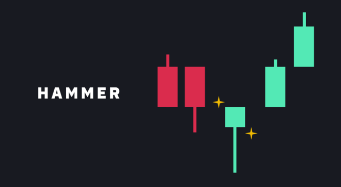
\includegraphics[width=0.5 \textwidth]{hammer.png}
		\caption{Młot}
		\label{fig:hammer}
		\textbf{Źródło:} \\
		\url{https://academy.binance.com/pl/articles/how-to-read-the-most-popular-crypto-candlestick-patterns}
	\end{figure}
	\vspace{12pt}
	
	\noindent \textbf{Odwrócony młot: \textit{(ang. inverted hammer)}}
	
	 Podobnie jak w przypadku młota, odwrócony młot charakteryzuje się górnym cieniem, który jest przynajmniej dwukrotnie dłuższy niż ciało. Pojawia się on na końcu trendu spadkowego i może wskazywać na potencjalny wzrost (Rysunek \ref{fig:ohammer}). \hyperref[info11]{[11]}
		\vspace{12pt}
	\begin{figure}[H]
		\centering
		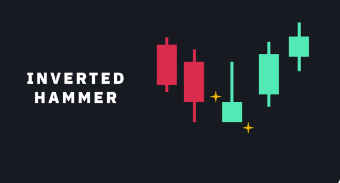
\includegraphics[width=0.5 \textwidth]{ohammer.png}
		\caption{Odwrócony młot}
		\label{fig:ohammer}
		\textbf{Źródło:} \\
		\url{https://academy.binance.com/pl/articles/how-to-read-the-most-popular-crypto-candlestick-patterns}
	\end{figure}
	\vspace{12pt}
	
	\noindent \textbf{Trzech białych żołnierzy: \textit{(ang. Three white soldiers)}}
	
	Formacja "Trzech białych żołnierzy" składa się z trzech zielonych świec, gdzie otwarcie kolejnej znajduje się w korpusie poprzedniej świecy, a zamknięcie każdej świecy jest wyższe niż cena maksymalna poprzedniej świecy. Długie korpusy i małe knoty świec wskazują na kontynuację trendu wzrostowego (Rysunek \ref{fig:Trzech białych żołnierzy}). \hyperref[info11]{[11]}
		\vspace{12pt}
	\begin{figure}[H]
		\centering
		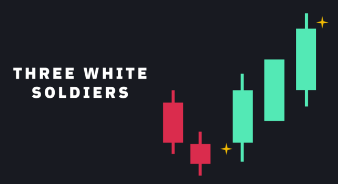
\includegraphics[width=0.5 \textwidth]{3zolnierzy.png}
		\caption{Trzech białych żołnierzy}
		\label{fig:Trzech białych żołnierzy}
		\textbf{Źródło:} \\
		\url{https://academy.binance.com/pl/articles/how-to-read-the-most-popular-crypto-candlestick-patterns}
	\end{figure}
	\vspace{12pt}
	
	\noindent \textbf{Trójka hossy: \textit{(ang. Rising three methods)}}
	
	 Charakteryzuje się kontynuacją trendu wzrostowego. Pierwsza świeca posiada duży korpus w porównaniu do cieni. Kolejne trzy świece spadkowe mają mały korpus i cienie, ale najważniejsze jest to, że mieszczą się one w zakresie pierwszej świecy. Ostatnia świeca, zielona, przewyższa maksymalne wartości czterech pozostałych świec (Rysunek \ref{fig:Trójka hossy}). \hyperref[info11]{[11]}
		\vspace{12pt}
	\begin{figure}[H]
		\centering
		\includegraphics[width=0.5 \textwidth]{Trojka hossy.png}
		\caption{Trójka hossy}
		\label{fig:Trójka hossy}
		\textbf{Źródło:} \\
		\url{https://academy.binance.com/pl/articles/how-to-read-the-most-popular-crypto-candlestick-patterns}
	\end{figure}
	\vspace{12pt}
	
	\noindent \textbf{Niedzwiedzie formacje świecowe:}
	\newline
	
	\noindent \textbf{Wisielec: \textit{(ang. Hanging man)}}
	
	 Jest to niedzwiedzi odpowiednik młota z małym korpusem i dużym, przynajmniej dwukrotnie wiekszym dolnym cieniem. Wystąpienie jego może oznaczać koniec trendu wzrostowego i przejęcie kontroli nad trendem niedzwiedzia (Rysunek \ref{fig:wisielec}). \hyperref[info11]{[11]}
		\vspace{12pt}
	\begin{figure}[H]
		\centering
		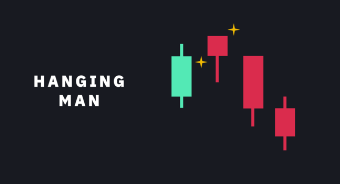
\includegraphics[width=0.5 \textwidth]{Wisielec.png}
		\caption{Wisielec}
		\label{fig:wisielec}
		\textbf{Źródło:} \\
		\url{https://academy.binance.com/pl/articles/how-to-read-the-most-popular-crypto-candlestick-patterns}
	\end{figure}
	\vspace{12pt}
	\noindent \textbf{Spadająca gwiazda: \textit{(ang. Shooting star)}}
	
	 Spadająca gwiazda charakteryzuje się brakiem bądź niewielkim dolnym knotem i dużym, przynajmniej dwukrotnie przewyższającym korpus, górnym knotem. Jest niedźwiedzim odpowiednikiem odwróconego młota i może oznaczać koniec trendu wzrostowego (Rysunek \ref{fig:spadająca gwiazda}). \hyperref[info11]{[11]}
	\vspace{12pt}
	\begin{figure}[H]
		\centering
		\includegraphics[width=0.5 \textwidth]{Shoting star.png}
		\caption{Spadająca gwiazda}
		\label{fig:spadająca gwiazda}
		\textbf{Źródło:} \\
		\url{https://academy.binance.com/pl/articles/how-to-read-the-most-popular-crypto-candlestick-patterns}
	\end{figure}
	\vspace{12pt}
	\noindent \textbf{Trzy czarne kruki: \textit{(ang.Three black crows)}}
	
	 Trzy czarne kruki charakteryzują się trzema świecami, gdzie otwarcie każdej kolejnej występuje w korpusie poprzedniej, a zamknięcie świecy jest coraz niżej niż poprzednia. Świece te nie powinny posiadać dużych knotów, co wskazuje na rosnącą podaż i spadek ceny (Rysunek \ref{fig:3kroki}). \hyperref[info11]{[11]}
	\vspace{12pt}
	\begin{figure}[H]
		\centering
		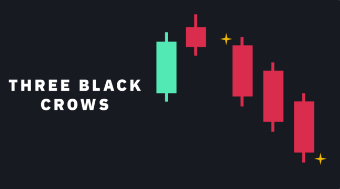
\includegraphics[width=0.5 \textwidth]{3kroki.png}
		\caption{Trzy czarne kruki}
		\label{fig:3kroki}
		\textbf{Źródło:} \\
		\url{https://academy.binance.com/pl/articles/how-to-read-the-most-popular-crypto-candlestick-patterns}
	\end{figure}
	\vspace{12pt}
	\noindent \textbf{Trójka bessy: \textit{(ang. Falling three methods)}}
	
	Odwrotność trójki hossy, sygnalizuje kontynuacje trendu spadkowego (Rysunek \ref{fig:Trójka bessy}). \hyperref[info11]{[11]}
	\vspace{12pt}
	\begin{figure}[H]
		\centering
		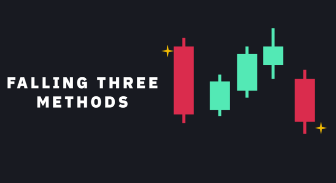
\includegraphics[width=0.5 \textwidth]{trojka bessy.png}
		\caption{Trójka bessy}
		\label{fig:Trójka bessy}
		\textbf{Źródło:} \\
		\url{https://academy.binance.com/pl/articles/how-to-read-the-most-popular-crypto-candlestick-patterns}
	\end{figure}
	\vspace{12pt}
	
	\noindent\textbf{Podsumowanie:}
	
	Przeanalizowaliśmy osiem formacji świecowych, które są najczęściej stosowane do identyfikacji trendów w kryptowalutach. Te formacje zostaną odpowiednio zaimplementowane do systemów uczenia maszynowego, aby przewidywać dalsze ruchy cenowe.
	\newline
	\section{Zniesienia Fibonacciego (Fibonacci Retracements)}
	
	Zniesienie Fibonacciego, inaczej znane jako ciąg Fibonacciego, jest jednym z podstawowych wskaźników używanych przez traderów i inwestorów. Ciąg ten zapoczątkował znany matematyk Leonardo Fibonacci w 1202 r\hyperref[info15]{[15]}. Zawiera liczby zwane liczbami Fibonacciego, które są wyrażone w postaci stosunków. Najważniejsze z nich to: 0\%,\ 23.6\%,\ 38.2\%,\ 61.8\%,\ 100\%,\ 138,2\%,\ 161,8\%. \hyperref[info14]{[14]}	\newline


	\subsection{Teoria ciągów Fibonacciego}

	\begin{definition}  
		Ciąg Fibonacciego to ciąg liczb naturalnych, w którym każdy kolejny wyraz ciągu jest sumą dwóch poprzednich. W przyjętej przez nas konwencji, pierwszy wyraz ciągu to 0, a drugi to 1. Formalnie można wyrazić to następująco \hyperref[info15]{[15]} :
	\end{definition}
	\vspace{12pt}
	\begin{equation}
		F_n = 
		\begin{cases} 
			0 & \text{dla } n = 0, \\
			1 & \text{dla } n = 1, \\
			F_{n-1} + F_{n-2} & \text{dla } n > 1.
		\end{cases}
	\label{eq:Fib}
	\end{equation}
	\vspace{12pt}
	
	\noindent Oto 20 pierwszych liczb z ciągu Fibonacciego: 
	\vspace{12pt}
	\setlength{\tabcolsep}{3pt}
	\begin{table}[h!]
		\centering
		\begin{tabular}{|c|c|c|c|c|c|c|c|c|c|c|c|c|c|c|c|c|c|c|c|}
			\hline
			$F_0$ & $F_1$ & $F_2$ & $F_3$ & $F_4$ & $F_5$ & $F_6$ & $F_7$ & $F_8$ & $F_9$ & $F_{10}$ & $F_{11}$ & $F_{12}$ & $F_{13}$ & $F_{14}$ & $F_{15}$ & $F_{16}$ & $F_{17}$ & $F_{18}$ & $F_{19}$\\
			\hline
			0 & 1 & 1 & 2 & 3 & 5 & 8 & 13 & 21 & 34 & 55 & 89 & 144 & 233 & 377 & 610 & 987 & 1597 & 2584 & 4451 \\
			\hline
		\end{tabular}
		\caption{Wartości liczb Fibonacciego od $F_0$ do $F_{19}$.}
		\textbf{Źródło: Opracowanie własne}
	\end{table}
	\vspace{12pt}
	\noindent Odpowiednie stosunki liczb tworzą odpowiednie poziomy Fibonacciego. \hyperref[info16]{[16]}\newline
	\begin{itemize}
		\item \textbf{0\% i 100\%} --- Są to ekstremalne punkty ruchu ceny, gdzie 0\% jest początkiem ruchu, a 100\% jego końcem.
		\item \textbf{61.8\%} --- Znany jako złota liczba, wynik podziału dowolnej liczby w ciągu przez liczbę następną (np. $\frac{21}{34} \approx 0.618$).
		\item \textbf{38.2\%} --- Jest przybliżeniem wyniku podziału dowolnej liczby w ciągu przez liczbę znajdującą się dwa miejsca dalej (np. $\frac{13}{34} \approx 0.382$).
		\item \textbf{23.6\%} --- Jest przybliżeniem wyniku podziału dowolnej liczby w ciągu przez liczbę znajdującą się trzy miejsca dalej (np. $\frac{377}{1597} \approx 0.236$).
		\item \textbf{138.2\%} --- Jest przybliżeniem wyniku podziału dowolnej liczby w ciągu przez liczbę znajdującą się dwa miejsca bliżej (np. $\frac{34}{13} \approx 1.382$).
		\item \textbf{161.8\%} --- Znany również jako złota liczba, wynik podziału dowolnej liczby w ciągu przez liczbę ją poprzedzającą (np. $\frac{34}{21} \approx 1.618$).\newline
	\end{itemize}

	
	\noindent Traderzy w analizie technicznej stosują również trzy dodatkowe poziomy. Są to: \newline
	
	\begin{itemize}
		\item \textbf{50\%} --- Reprezentuje punkt równowagi lub symetrii. 
		\item \textbf{78.6\%} --- Pochodzi z pierwiastka kwadratowego złotej liczby ,
		\item \textbf{88.6\%} --- Jest to mniej powszechny poziom, który czasem jest używany i wynika z pierwiastka kwadratowego z 0.786.
	\end{itemize}
	
	\subsection{Zastosowanie zniesień Fibonacciego}
	
	Zastosowanie zniesień Fibonacciego posiada ogromne znaczenie w analizie technicznej. Aby nanieść te poziomy, należy wybrać przedział, w którym znajduje się ruch cenowy: od lokalnego minimum do lokalnego maksimum (w przypadku trendu wzrostowego) lub od lokalnego maksimum do lokalnego minimum (w przypadku trendu spadkowego). Wyznaczenie tych poziomów ma duże znaczenie jako potencjalne punkty wsparcia i oporu. Punkt wsparcia tworzy się, kiedy cena zbliża się do poziomu od dołu; następuje wsparcie, co oznacza, że podaż może maleć i następuje odbicie od tego poziomu. Podobnie w przypadku oporu: kiedy cena zbliża się od góry do poziomu, popyt może maleć i cena zawraca, tworząc punkt oporu.
	
	Na Rysunku \ref{fig:ciagf} został przedstawiony przykład użycia poziomów Fibonacciego. Białą linią zostały zaznaczone najbardziej znaczące poziomy wsparcia. Gdy cena BTC zbliżała się do tych poziomów, następowało odbicie ceny w przeciwnym kierunku. Kolorem żółtym zaznaczono poziomy oporów; widać, że cena odbiła się od tych poziomów. We wszystkich innych przypadkach, gdy cena przebiła dany poziom wsparcia lub oporu, nastąpiła zmiana funkcji tego poziomu odpowiednio na potencjalny opór lub wsparcie.
	
	Aby wyznaczyć poziomy zniesień Fibonacciego dla danej ceny \( P_t \), gdzie \( t \) jest indeksem czasu, w pierwszej kolejności należy dokonać identyfikacji dwóch skrajnych punktów ruchu cenowego na wykresie. Rozpatrując pewien przedział czasowy i zakładając wyznaczenie:
	
	\[
	P_{\text{min}} = \min(P_t) \quad \text{oraz} \quad P_{\text{max}} = \max(P_t),
	\]
	
	dla wszystkich \( t \) w wybranym przedziale. Jeśli mamy do czynienia z trendem wzrostowym, zostało przyjęte, że ruch cenowy rozpoczął się na poziomie minimalnym \( P_{\text{min}} \), a zakończył (lub osiągnął szczyt) na poziomie maksymalnym \( P_{\text{max}} \).
	
	Po zidentyfikowaniu tych wartości można obliczyć tzw. poziomy zniesień Fibonacciego, bazując na ustalonych współczynnikach, które najczęściej wynoszą \( 23{,}6\% \), \( 38{,}2\% \), \( 50\% \), \( 61{,}8\% \) oraz \( 78{,}6\% \). W zapisie dziesiętnym są to odpowiednio:
	
	\[
	F_{23{,}6\%} = 0{,}236, \quad F_{38{,}2\%} = 0{,}382, \quad F_{50\%} = 0{,}500, \quad F_{61{,}8\%} = 0{,}618, \quad F_{78{,}6\%} = 0{,}786.
	\]
	
	Dla trendu wzrostowego poziomy zniesień są definiowane następująco:
	
	\[
	P_{\text{fib}}(F) = P_{\text{min}} + (P_{\text{max}} - P_{\text{min}}) \cdot F,
	\]
	
	gdzie \( F \) jest jednym z powyższych współczynników (np. \( 0{,}236 \), \( 0{,}382 \), \( 0{,}500 \), \( 0{,}618 \), \( 0{,}786 \)). Oznacza to, że jeśli cena maksymalna osiągnęła poziom \( P_{\text{max}} \), a minimalna wynosi \( P_{\text{min}} \), to zniesienie o \( 61{,}8\% \) (czyli \( F=0{,}618 \)) będzie na poziomie:
	
	\[
	P_{\text{fib}}(0{,}618) = P_{\text{min}} + (P_{\text{max}} - P_{\text{min}}) \cdot 0{,}618.
	\]
	
	Analogicznie, dla pozostałych współczynników otrzymujemy pozostałe poziomy zniesień. Każdy z tych poziomów może pełnić rolę potencjalnego wsparcia lub oporu. Jeśli po osiągnięciu pewnego maksimum cena zaczyna spadać i dochodzi do poziomu \( P_{\text{fib}}(F) \), może on zadziałać jako punkt wsparcia, od którego cena odbije się w górę. W przypadku zbliżania się ceny do poziomu od dołu, poziom ten może zadziałać jako opór, utrudniając dalszy wzrost ceny. W sytuacjach, gdy poziom wsparcia lub oporu zostanie trwale przełamany, jego rola może ulec odwróceniu — dawne wsparcie może stać się oporem i odwrotnie.

	\vspace{12pt}
	\begin{figure}[H]
		\centering
		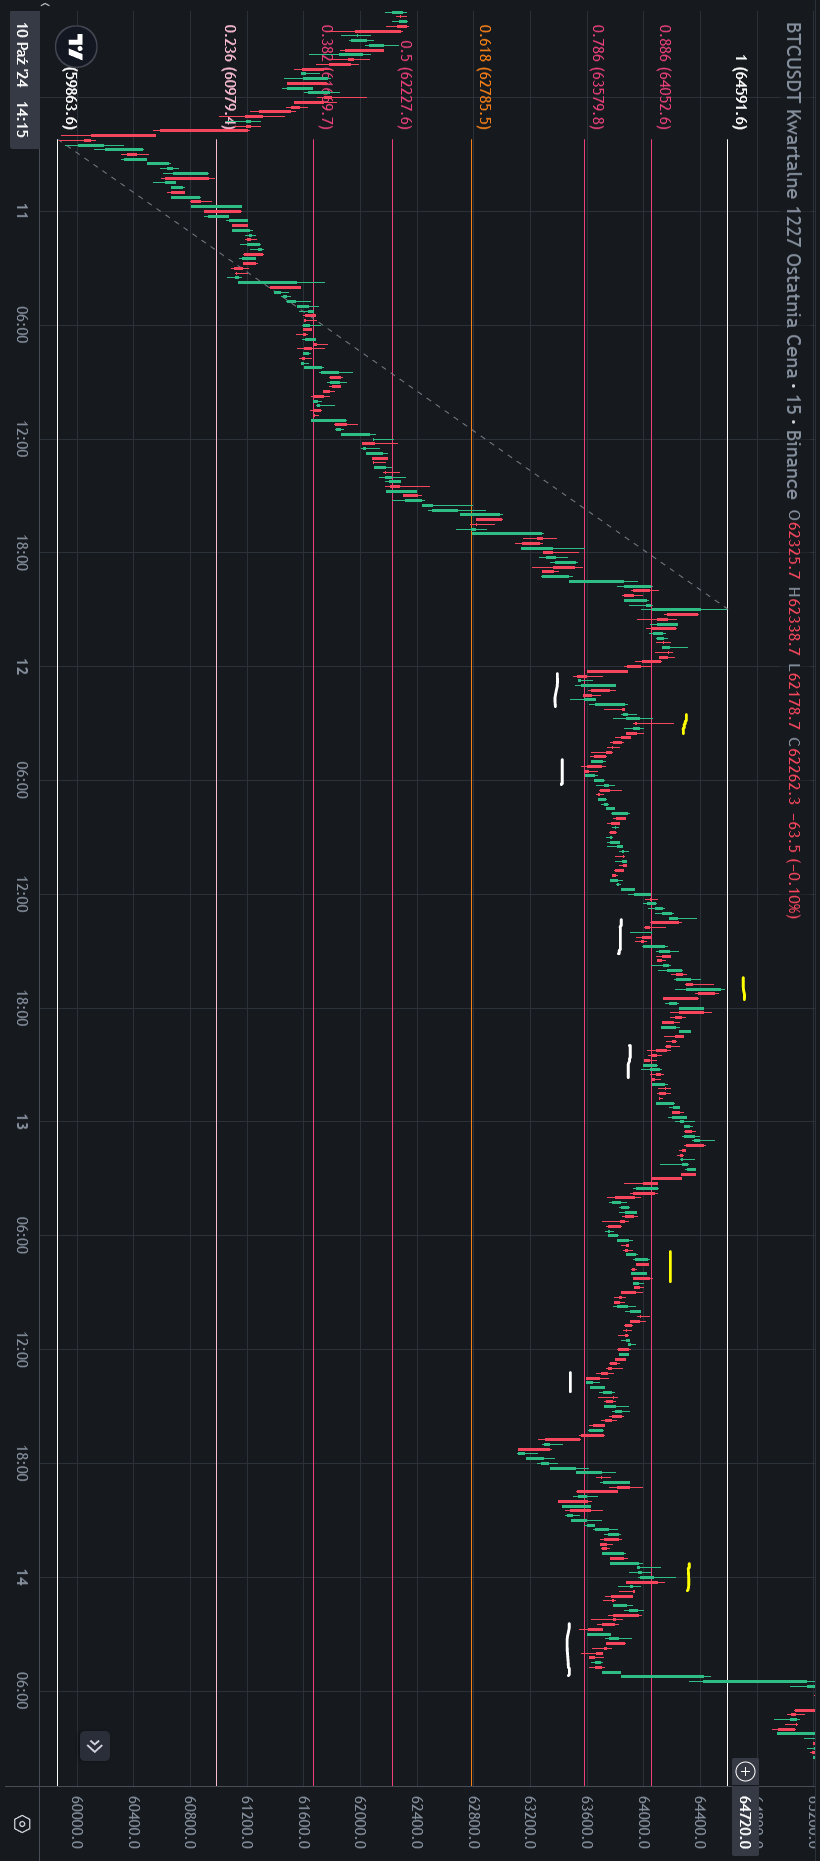
\includegraphics[width=0.55\textwidth]{fibo.png}
		\caption{Przykład użycia zniesienia Fibonacciego kryptowaluty BTC na giełdzie Binance.}
		\label{fig:ciagf}
		\textbf{Źródło: Opracowanie własne} 	\end{figure}
	\vspace{12pt}
	
	\section{Oscylator stochastyczny \textit{(ang. Stochastic Oscillator)}}
	Ostatnim analizowanym wskaźnikiem analizy technicznej jest oscylator stochastyczny, stworzony w latach 50. XX wieku. Do dziś jest używany przez traderów ze względu na jego skuteczność. Dzięki szybkiemu reagowaniu, oscylator dostarcza wielu sygnałów, umożliwiających szybkie i efektywne podejmowanie decyzji. \hyperref[info17]{[17]}\newline

	\subsection{Opis oscylatora}
	
	Oscylator stochastyczny (\textit{ang. Stochastic Oscillator}), STS, jest wskaźnikiem \textit{momentum}, tzn. pozwala określić siłę, z jaką rynek podąża w danym momencie. Oscylator działa na zasadzie porównywania aktualnej ceny zamknięcia z cenami zamknięcia z określonego okresu. Podczas trendu spadkowego ceny oscylują przy dolnej granicy zakresu, a przy trendzie wzrostowym przy górnej \hyperref[info17]{[17]}. Do obliczenia wskaźnika stochastycznego potrzebne są: 
	\begin{itemize}
		\item ceny minimalne z danego okresu,
		\item ceny maksymalne z danego okresu,
		\item cena zamknięcia z bieżącego okresu.
	\end{itemize}
	
	\noindent Wzór na obliczenie wartości wskaźnika STS:
	\begin{equation}
		\%K_t = \left( \frac{C_t - L_n}{H_n - L_n} \right) \times 100,
		\label{eq:OS}
	\end{equation}
	gdzie: \\
	\( C_t \) – aktualna cena zamknięcia, \\
	\( L_n \) – najniższa cena z ostatnich \( n \) okresów, \\
	\( H_n \) – najwyższa cena z ostatnich \( n \) okresów. \newline
	
	\noindent 
	 Otrzymujemy w ten sposób linię \%K, nazywaną wolnym oscylatorem stochastycznym. Do pełnego działania oscylatora potrzebna jest jeszcze druga linia \%D, nazywana szybkim oscylatorem stochastycznym, będąca 3-okresową średnią kroczącą wartości \%K. Wzór na linię \%D:
	 \begin{equation}
	 	\%D_t = \frac{1}{3} \sum_{i=0}^{2} \%K_{t - i},
	 	\label{eq:D}
	 \end{equation}

	Wartości obu tych linii mieszczą się w przedziale od 0 do 100. W celu dobrej interpretacji sygnałów generowanych przez oscylator, tworzone są dwie poziome linie, odpowiednio na wartościach 20 i 80. Przedział od 0 do 20 oznacza sygnał wykupienia rynku, a od 80 do 100 sygnał wyprzedania rynku . \hyperref[info17]{[17]} 

	\subsection{Sygnały generowane przez oscylator:}
	 \textbf{a)} Na rysunku \ref{fig:OSa} zaprezentowano wykres ceny Bitcoin w parze do Polskiego Złotego z giełdy MTGOX wraz z dolnym panelem, na którym znajduje się oscylator stochastyczny. Oscylator ten pokazuje relację ostatniej ceny zamknięcia do zakresu cen w danym okresie i jest wykorzystywany do identyfikacji stanów wykupienia (\emph{ang. overbought}) i wyprzedania (\textit{ang. oversold}) na rynku. Na rysunku zaznaczono przykładowe momenty, w których oscylator generuje sygnały kupna (zielona strzałka) i sygnay sprzedaży (czerwoan strzałka). Linią niebieską została narysowana linia \% K, a czerwoną linia \% D. Sygnał możemy interpretować na 3 różne sposoby:
	
	\begin{itemize} 
		\item Kiedy linia \% K przetnie od góry poziom 80, jest to znak dla inwestorów do sprzedaży aktywa. 
		\item Kiedy linia \% K przetnie od dołu poziom 20, jest to znak dla inwestorów do kupna aktywa. 
	\end{itemize}
	\vspace{12pt}
	\begin{figure}[H]
		\centering
		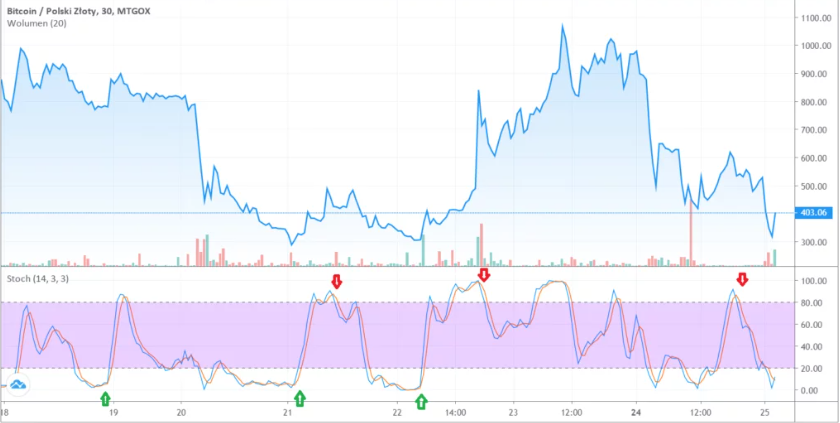
\includegraphics[width=1\textwidth]{STSa.png}
		\caption{Sygnały kupna/sprzedaży generowane przez STS.}
		\label{fig:OSa}
		\textbf{Źródło:}\
		\url{https://gieldomania.pl/oscylator-stochastyczny-interpretacja/}
	\end{figure}
	\vspace{12pt}	 	
	 
	\noindent \textbf{b)} Drugim sposobem na generowanie sygnału jest przecięcie lini. 
	 
	\begin{itemize} 
	 	\item Kiedy linia \% K przetnie od góry lini \% D, jest to znak dla inwestorów do sprzedaży aktywa. 
	 	\item Kiedy linia \% K przetnie od dołu lini \% D, jest to znak dla inwestorów do kupna aktywa. 
	\end{itemize}
	
	 	
	\noindent \textbf{c)} 
	Ostatnim sposobem jest zależność pomiędzy kształtowaniem się dołków (minimów) na wykresie cenowym, a dołkami na oscylatorze STS. Jest to klasyczna analiza dywergencji, która polega na porównywaniu kierunku zmian oscylatora z kierunkiem zmian ceny:. 
	\begin{itemize} 
		\item Wzrost minimów na oscylatorze przy spadających minimach na cenie (dywergencja bycza):
		Jeśli na wykresie cenowym widzimy, że kolejne dołki cenowe są coraz niżej (trend spadkowy), ale jednocześnie odpowiadające im minima na oscylatorze STS układają się coraz wyżej, jest to tzw. dywergencja bycza. Oznacza to, że chociaż cena dalej spada, to momentum spadkowe słabnie. Taka sytuacja często poprzedza zmianę trendu – w tym przypadku może sygnalizować koniec spadków i rozpoczęcie trendu wzrostowego  \ref{fig:OSc}.	
		\item  Spadek minimów na oscylatorze przy rosnących minimach na cenie (dywergencja niedzwiedzia):
		Jeśli cena notuje coraz wyższe dołki , ale minima na STS obniżają się, wówczas pojawia się dywergencja niedźwiedzia. Mimo rosnącej ceny, wewnętrzna siła rynku mierzona przez STS słabnie, co może być sygnałem, koniec trendu wzrostowego.
	\end{itemize}
	\vspace{12pt}
	\begin{figure}[H]
		\centering
		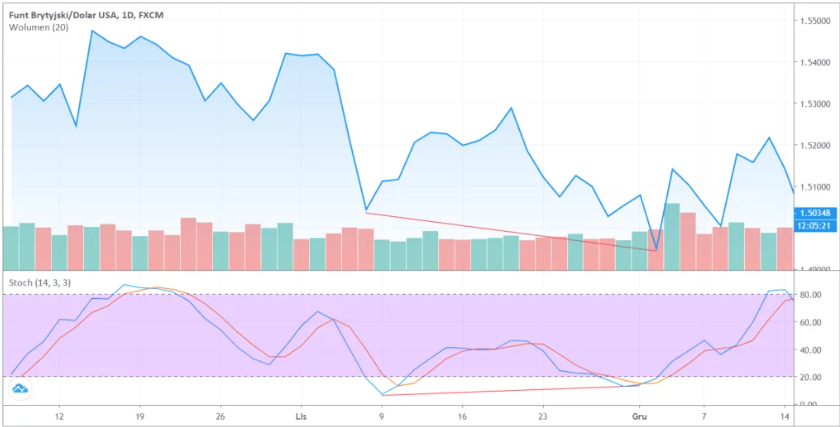
\includegraphics[width=1\textwidth]{OSc.png}
		\caption{Sygnały kupna/sprzedaży generowane przez STS.}
		\label{fig:OSc}
		\textbf{Źródło:}\
		\url{https://gieldomania.pl/oscylator-stochastyczny-interpretacja/}
	\end{figure}
	\vspace{12pt}
	 Ważne jest, aby sygnały generowane przez oscylator stochastyczny, były w przedziałach od 0 do 20 lub od 80 do 100. Wtedy jesteśmy pewni, że jakość sygnału generowanego przez STS będzie najwyższa. \hyperref[info15]{[15]}
	 	
	 	

	% Metody uczenia maszynowego w prognozowaniu kursów kryptowalut
	\chapter{Metody uczenia maszynowego w prognozowaniu kursów kryptowalut}
	
	Ten rozdział pozwala zagłębić się w metode uczenia maszynowego wykorzystywaną do predykcji cen kryptowalut. Program został stworzony w języku programowania Python z wykorzystaniem modelu XGBOOST, pochodząca z biblioteki xgboost. Przechodząc dalej, wyjaśnimy podstawowe pojęcia związane z tym modelem. \newline
	
	\begin{definition} 
	   \emph{"XGBoost, co oznacza Extreme Gradient Boosting, to skalowalny, rozproszony wzmocniony gradientem biblioteka do uczenia maszynowego drzewa decyzyjnego (GBDT). Zapewnia równoległe wzmocnienie drzewa i jest wiodącą biblioteką uczenia maszynowego dla problemów regresji, klasyfikacji i rankingu."} \hyperref[info21]{[21]}
	\end{definition}

	\begin{definition} 
		\textit{drzewo decyzyjne – graficzna metoda wspomagania procesu decyzyjnego, stosowana w teorii decyzji} \hyperref[info23]{[23]}
	\end{definition}

	\begin{definition} 
		\textit{Gradient – pole wektorowe wskazujące kierunki najszybszych wzrostów wartości danego pola skalarnego.} \hyperref[info22]{[22]}
	\end{definition}
	
	Załóżmy, że chcemy zoptymalizować strategię handlu kryptowalutami, aby maksymalizować zyski przy jednoczesnym minimalizowaniu ryzyka strat. Każda decyzja w strategii handlowej reprezentuje określone działanie, takie jak kupno, sprzedaż lub trzymanie danej kryptowaluty. W tej sytuacji można użyć funkcji kosztu \( C(w) \), która określa poziom ryzyka strategii w zależności od parametrów \( w \) przypisanych poszczególnym działaniom handlowym.
	
	Gradient tej funkcji kosztu wskazałby najbardziej efektywny kierunek zmiany parametrów strategii, aby zminimalizować ryzyko przy zachowaniu oczekiwanych zysków. Jednak podążając za gradientem, moglibyśmy natrafić na lokalne minimum – na przykład strategię, która optymalizuje zyski tylko w krótkim okresie, ale nie uwzględnia długoterminowych trendów rynkowych kryptowalut. To pokazuje, jak gradient może prowadzić do ulepszeń, ale również może wprowadzać w błąd poprzez skupienie się na lokalnych, a nie globalnych rozwiązaniach.
	
	\begin{definition} 
		\textit{Boosting to tak zwane przyśpieszenie. Polega na tym, że w każdym kolejnym kroku chcemy poprawić wcześniejsze błędy.} \hyperref[info22]{[22]}
	\end{definition}
	
	Modelu XGBOOST wykorzystuje proste drzewo decyzyjne. Przechodząc po kolejnych iteracjach, nasze drzewa decyzyjne próbują naprawić błędy poprzedniego. Dzięki gradientowi, wiemy w którą strone podążać. Jest to idea przyśpieszonego uczenia. Rysunki : przedstawiają w kolejnych krokach zasade działania XGBOOSTER-a  \hyperref[info22]{[22]} \newline
	
	\textbf{Podstawowe hiperparametry}
	\begin{itemize}
		\item \textbf{learning\_rate / eta [default=0.3]} - rozmiar kroku do kolejnej iteracji.
		\item \textbf{max\_depth [default=6]} - maksymalna głębokość drzew decyzyjnych.
		\item \textbf{n\_estimators} - liczba skonstruowanych drzew w modelu.
		\item \textbf{min\_child\_weight} - minimalna liczba obserwacji wymagana w każdym z liści drzewa.
		\item \textbf{gamma [default=0]} - parametr zmniejszający straty potrzebne do stworzenia kolejnego węzła w drzewie.
		\item \textbf{subsample [default=1]} - procent obserwacji używanych do budowy każdego drzewka.
		\item \textbf{colsample\_bytree [default=1]} - procent cech używanych do budowy prostego drzewa.
	\end{itemize}

	% Eksperymenty i wyniki
	\chapter{Eksperymenty i wyniki}
	W swojej pracy przeanalizowałem każdy wskaźnik analizy techniczej. Wyniki posłużyły mi jako dane wejsciowe do modelu predykcji.
	
	\textbf{Średnia ruchoma prosta}
	Przeanalizowałem podwójną średnią kroczącą prostą w celu sprawdzenia, która maksymalizuje zyski. Sprawdziłem kombinacje krótkoterminowej sredniej kroczącej z przedziału $[1-50]$ i długoterminową z przedziału $[100-200]$ dla cen zamknięcia świec. W rezultacie najbardziej optymalnme sygnały kupna/sprzedaży średnich kroczących to połączenie SMA5 z SMA104. Przy zainwestowaniu 1000 dolarów na początku okresu ta oto średnia przyniosła najlepszy zysk. Stowrzone zostały również średnie kroczące dla ceny otwarcia, max i min w celu wykorzystania wyników do modelu predykcji każdej świecy. Rysunek \ref{fig:SMA} przedstawiaja podwójną srednią kroczącą dla ceny zamknięcia naniesiongo na wykres BTC. 
	\vspace{12pt}
	\begin{figure}[H]
		\centering
		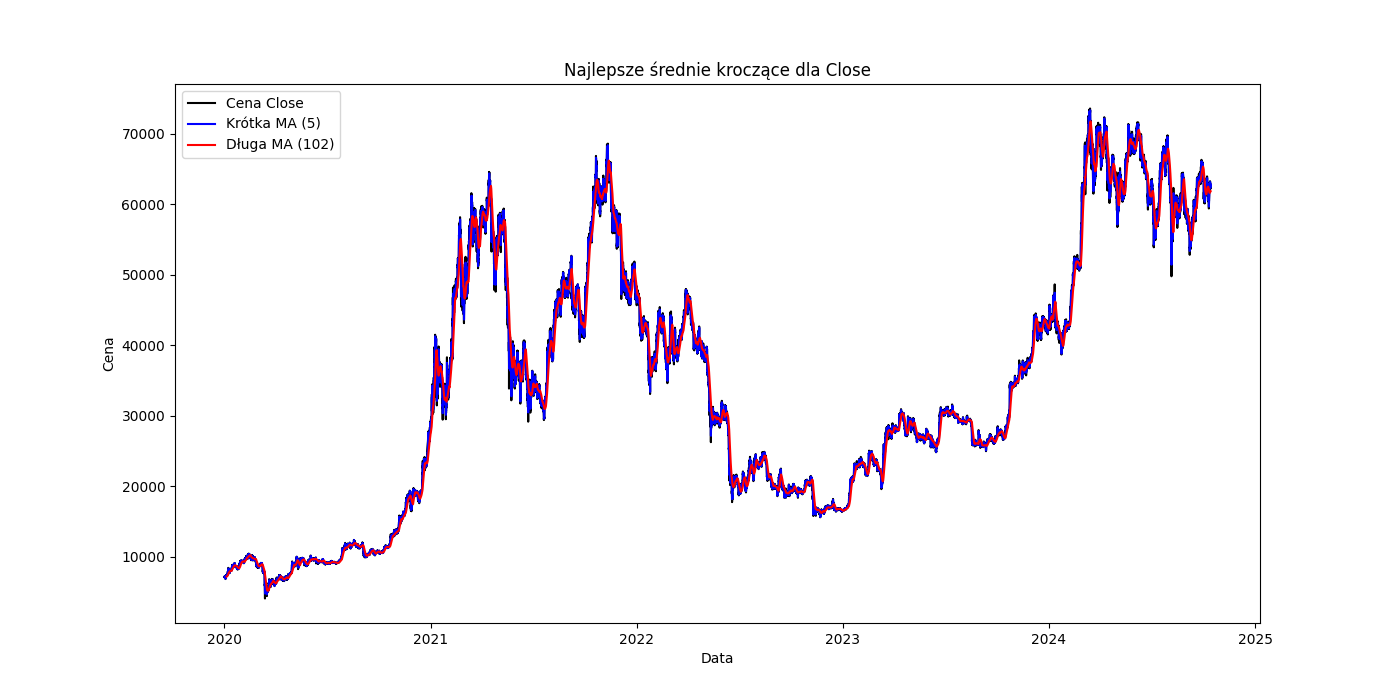
\includegraphics[width=1 \textwidth]{Najlepszy wynik dla 2 srednich kroczacych SMA 102 i 5.png}
		\caption{Najlepszy wynik dla podwójnej średniej kroczącej SMA 102 i SMA5}
		\label{fig:SMA}
		\textbf{Źródło: Opracowanie własne} \\
	\end{figure}
	\vspace{12pt}

	
	
	
	
	
	
	
	
	
	
	
	
	
	\vspace{12pt}
	% Dyskusja
	\chapter{Dyskusja}
	% Podsumowanie i wnioski
	\chapter{Podsumowanie i wnioski}
	% Bibliografia
	\bibliographystyle{plain}
	\bibliography{references}
	% Dodatki
	\appendix
\hangindent=1.5em
\noindent \textbf{[1]} \href{https://kriptomat.io/pl/finanse-i-inwestycje/jakie-sa-kluczowe-elementy-analizy-fundamentalnej-w-handlu-kryptowalutami/}{Kriptomat} \newline

\noindent \textbf{[2]} Adam Zaremba pt. \textit{"Giełda Podstawy inwestowania"}, wydanie 3 zaktualizowane Copyright \textcopyright{} Adam Zaremba 2014, 2022 \newline

\noindent \textbf{[3]} Krzysztof Kochan pt. \textit{"Analiza techniczna w praktyce"} Copyright \textcopyright{} Helion SA 2020 \newline

\noindent \textbf{[4]} \href{https://pl.wikipedia.org/wiki/Kryptowaluta}{Wikipedia: Kryptowaluta} \newline

\noindent \textbf{[5]} \href{https://www.investopedia.com/terms/c/cryptocurrency.asp}{Investopedia: Cryptocurrency} \newline

\noindent \textbf{[6]} \href{https://www.forbes.com/advisor/investing/cryptocurrency/}{Forbes: Cryptocurrency} \newline

\noindent \textbf{[7]} \href{https://przemyslprzyszlosci.gov.pl/nawigator-technologiczny/blockchain/}{Przemysł Przyszłości: Blockchain} \newline

\noindent \textbf{[8]} \href{https://www.parkiet.com/kryptowaluty/art40380371-gdzie-sa-globalne-centra-wiary-w-wirtualne-waluty}{Parkiet: Globalne centra wirtualnych walut} \newline

\noindent \textbf{[9]} \href{https://pl.wikipedia.org/wiki/Ethereum}{Wikipedia: Ethereum} \newline

\noindent \textbf{[10]} \href{https://businessinsider.com.pl/kryptowaluty/koparka-kryptowalut}{Business Insider: Koparka kryptowalut} \newline

\noindent \textbf{[11]} \href{https://academy.binance.com/pl/articles/how-to-read-the-most-popular-crypto-candlestick-patterns}{Binance Academy: Candlestick Patterns} \newline

\noindent \textbf{[12]} \href{https://edukacjagieldowa.pl/gieldowe-abc/samouczki/formacje-swiecowe-kontynuacji}{Edukacja Giełdowa: Formacje Świecowe Kontynuacji} \newline

\noindent \textbf{[13]} \href{https://pl.wikipedia.org/wiki/%C5%9Awiece_japo%C5%84skie}{Wikipedia: Świece Japońskie} \newline

\noindent \textbf{[14]} Technical Analysis of Digital Currencies and the M \newline

\noindent \textbf{[15]} \href{https://pl.wikipedia.org/wiki/Ci%C4%85g_Fibonacciego}{Wikipedia: Ciąg Fibonacciego} \newline

\noindent \textbf{[16]} \href{https://edukacjagieldowa.pl/gieldowe-abc/samouczki/zniesienia-fibonacciego}{Edukacja Giełdowa: Zniesienia Fibonacciego} \newline

\noindent \textbf{[17]} \href{https://gieldomania.pl/oscylator-stochastyczny-interpretacja/}{Giełdomania: Oscylator Stochastyczny} \newline

\noindent \textbf{[18]} \href{https://admiralmarkets.com/pl/education/articles/forex-indicators/srednia-ruchoma-prosta}{Admiral Markets: Średnia Ruchoma Prosta} \newline

\noindent \textbf{[19]} \href{https://pl.wikipedia.org/wiki/Uczenie_maszynowe}{Wikipedia: Uczenie maszynowe}\newline

\noindent \textbf{[20]} \href{https://www.sap.com/poland/products/artificial-intelligence/what-is-machine-learning.html}{Czym jest uczenie maszynowe?}\newline

\noindent \textbf{[21]} \href{https://www.nvidia.com/en-us/glossary/xgboost/}{XGBOOST}\newline

\noindent \textbf{[22]} \href{https://miroslawmamczur.pl/czym-jest-wzmocnienie-gradientowe-gradient-boosting-i-dlaczego-jest-taki-dobry/}{Czym jest wzmocnienie gradientowe?}\newline

\noindent \textbf{[23]} \href{https://pl.wikipedia.org/wiki/Drzewo_decyzyjne}{Drzewa decyzyjne}\newline
	\chapter{Załączniki}
	\chapter{DODATKI} \addcontentsline{toc}{chapter}{DODATKI}

\end{document}